\documentclass[journal,12pt,twocolumn]{IEEEtran}

\usepackage{setspace}
\usepackage{gensymb} 

\singlespacing


\usepackage[cmex10]{amsmath}

\usepackage{amsthm}


\usepackage{mathrsfs}
\usepackage{txfonts}
\usepackage{stfloats}
\usepackage{bm}
\usepackage{cite}
\usepackage{cases}
\usepackage{subfig}

\usepackage{longtable}
\usepackage{multirow}

\usepackage{enumitem}
\usepackage{mathtools}
\usepackage{steinmetz}
\usepackage{tikz}
\usepackage{circuitikz}
\usepackage{verbatim}
\usepackage{tfrupee}
\usepackage[breaklinks=true]{hyperref}
\usepackage{graphicx}
\usepackage{tkz-euclide}

\usetikzlibrary{calc,math}
\usepackage{listings}
    \usepackage{color}                                            %%
    \usepackage{array}                                            %%
    \usepackage{longtable}                                        %%
    \usepackage{calc}                                             %%
    \usepackage{multirow}                                         %%
    \usepackage{hhline}                                           %%
    \usepackage{ifthen}                                           %%
    \usepackage{lscape}     
\usepackage{multicol}
\usepackage{chngcntr}

\DeclareMathOperator*{\Res}{Res}

\renewcommand\thesection{\arabic{section}}
\renewcommand\thesubsection{\thesection.\arabic{subsection}}
\renewcommand\thesubsubsection{\thesubsection.\arabic{subsubsection}}

\renewcommand\thesectiondis{\arabic{section}}
\renewcommand\thesubsectiondis{\thesectiondis.\arabic{subsection}}
\renewcommand\thesubsubsectiondis{\thesubsectiondis.\arabic{subsubsection}}


\hyphenation{op-tical net-works semi-conduc-tor}
\def\inputGnumericTable{}                                 %%

\lstset{
%language=C,
frame=single, 
breaklines=true,
columns=fullflexible
}
\begin{document}


\newtheorem{theorem}{Theorem}[section]
\newtheorem{problem}{Problem}
\newtheorem{proposition}{Proposition}[section]
\newtheorem{lemma}{Lemma}[section]
\newtheorem{corollary}[theorem]{Corollary}
\newtheorem{example}{Example}[section]
\newtheorem{definition}[problem]{Definition}

\newcommand{\BEQA}{\begin{eqnarray}}
\newcommand{\EEQA}{\end{eqnarray}}
\newcommand{\define}{\stackrel{\triangle}{=}}
\bibliographystyle{IEEEtran}
\providecommand{\mbf}{\mathbf}
\providecommand{\pr}[1]{\ensuremath{\Pr\left(#1\right)}}
\providecommand{\qfunc}[1]{\ensuremath{Q\left(#1\right)}}
\providecommand{\sbrak}[1]{\ensuremath{{}\left[#1\right]}}
\providecommand{\lsbrak}[1]{\ensuremath{{}\left[#1\right.}}
\providecommand{\rsbrak}[1]{\ensuremath{{}\left.#1\right]}}
\providecommand{\brak}[1]{\ensuremath{\left(#1\right)}}
\providecommand{\lbrak}[1]{\ensuremath{\left(#1\right.}}
\providecommand{\rbrak}[1]{\ensuremath{\left.#1\right)}}
\providecommand{\cbrak}[1]{\ensuremath{\left\{#1\right\}}}
\providecommand{\lcbrak}[1]{\ensuremath{\left\{#1\right.}}
\providecommand{\rcbrak}[1]{\ensuremath{\left.#1\right\}}}
\theoremstyle{remark}
\newtheorem{rem}{Remark}
\newcommand{\sgn}{\mathop{\mathrm{sgn}}}
\providecommand{\abs}[1]{\left\vert#1\right\vert}
\providecommand{\res}[1]{\Res\displaylimits_{#1}} 
\providecommand{\norm}[1]{\left\lVert#1\right\rVert}
%\providecommand{\norm}[1]{\lVert#1\rVert}
\providecommand{\mtx}[1]{\mathbf{#1}}
\providecommand{\mean}[1]{E\left[ #1 \right]}
\providecommand{\fourier}{\overset{\mathcal{F}}{ \rightleftharpoons}}
%\providecommand{\hilbert}{\overset{\mathcal{H}}{ \rightleftharpoons}}
\providecommand{\system}{\overset{\mathcal{H}}{ \longleftrightarrow}}
	%\newcommand{\solution}[2]{\textbf{Solution:}{#1}}
\newcommand{\solution}{\noindent \textbf{Solution: }}
\newcommand{\cosec}{\,\text{cosec}\,}
\providecommand{\dec}[2]{\ensuremath{\overset{#1}{\underset{#2}{\gtrless}}}}
\newcommand{\myvec}[1]{\ensuremath{\begin{pmatrix}#1\end{pmatrix}}}
\newcommand{\mydet}[1]{\ensuremath{\begin{vmatrix}#1\end{vmatrix}}}
\numberwithin{equation}{subsection}
\makeatletter
\@addtoreset{figure}{problem}
\let\StandardTheFigure\figure
\let\vec\mathbf
\renewcommand{\thefigure}{\theproblem}
\def\putbox#1#2#3{\makebox[0in][l]{\makebox[#1][l]{}\raisebox{\baselineskip}[0in][0in]{\raisebox{#2}[0in][0in]{#3}}}}
     \def\rightbox#1{\makebox[0in][r]{#1}}
     \def\centbox#1{\makebox[0in]{#1}}
     \def\topbox#1{\raisebox{-\baselineskip}[0in][0in]{#1}}
     \def\midbox#1{\raisebox{-0.5\baselineskip}[0in][0in]{#1}}
\vspace{3cm}
\title{ASSIGNMENT-3}
\author{D.Ravalika}
\maketitle
\bigskip
\renewcommand{\thefigure}{\theenumi}
\renewcommand{\thetable}{\theenumi}
Download all python codes from 
\begin{lstlisting}
https://github.com/Ravalika1630/Assignment-3/blob/main/assignment3.py
\end{lstlisting}
%
and latex-tikz codes from 
%
\begin{lstlisting}
https://github.com/Ravalika1630/Assignment-3/blob/main/Assignment%203.tex

\end{lstlisting}
%
\section{QUESTION NO-2.30}

\item Draw JUMP with JU=3.5, UM=4, MP=5,PJ=4.5 and PU=6.5 .
%
\section{SOLUTION}
 Given,
\begin{align}
\ JU=3.5, UM=4, MP=5, PJ=4.5, PU=6.5 .
\end{align}
Now,
\begin{align}
JU=\norm{\vec{J}-\vec{U}} = 3.5
 \\
UM=\norm{\vec{U}-\vec{M}} = 4
 \\
MP=\norm{\vec{M}-\vec{p}} = 5
 \\
PJ=\norm{\vec{P}-\vec{J}} = 4.5
 \\
PU=\norm{\vec{P}-\vec{U}} = 6.5
\end{align}
\begin{enumerate}
\item We know,a quadrilateral is a polygon with 4 sides if we have four points they will not form a quadrilateral if any three points are collinear. 
$\triangle PMU$ and $\triangle PJU$ are two triangles of given quadrilateral.
Let us consider $\triangle PMU$-
\begin{align}
\norm{\vec{U}-\vec{M}}+\norm{\vec{P}-\vec{U}}&=10.5> \norm{\vec{M}-\vec{P}}\\
\norm{\vec{P}-\vec{U}}+\norm{\vec{M}-\vec{P}}&=11.5>\norm{\vec{U}-\vec{M}}\\
\norm{\vec{U}-\vec{M}}+\norm{\vec{M}-\vec{P}}&=10>\norm{\vec{P}-\vec{U}}
\end{align}
Triangle inequality is satisfied.
$\therefore$ $\triangle PMU$ can be constructed.
Similarly, Now we consider $\triangle PJU$
\begin{align}
\norm{\vec{P}-\vec{J}} + \norm{\vec{J}-\vec{U}}&=8.0 > \norm{\vec{P}-\vec{U}}
\\
\norm{\vec{J}-\vec{U}} + \norm{\vec{P}-\vec{U}}&=10.0 > \norm{\vec{P}-\vec{J}}
\\
\norm{\vec{P}-\vec{U}} + \norm{\vec{P}-\vec{J}}&=11.0 > \norm{\vec{J}-\vec{U}}
\end{align}
Triangle inequality is satisfied.
$\therefore$ $\triangle PJU$ can be constructed.
$\therefore$ Given sides form a quadrilateral.
Vertices of quadrilateral JUMP:
Now from $\triangle PJU$ ,the sides of $\triangle PJU$ are known Which means vertices P,J and U can be obtained using example 1.3
Similarly,the vertices of $\triangle PJU$ can be obtained using example 1.3
$\therefore$ Vertices of given Quadrilateral JUMP can be written as,
\begin{align}
\vec{P}=\myvec{0\\0},\vec{J} = \myvec{4.5\\0}, \vec{U}=\myvec{5.58\\3.33},\vec{M}=\myvec{3.94\\3.07}
\end{align}
Plot of the Quadrilateral JUMP :
\numberwithin{figure}{section}
\begin{figure}[!ht]
    \centering
    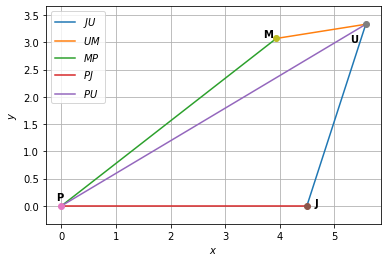
\includegraphics[width=\columnwidth]{JUMP fig.png}
    \caption{Quadrilateral JUMP}
    \label{fig:Quadrilateral JUMP}
\end{figure}
\end{enumerate}
\end{document}